\chapter{Metody přistávání} \label{chap:algs}
    Součástí této práce je návrh systému pro simulaci přistání bezpilotního letounu na plošině, který umožňuje implementovat libovolnou metodu navádění letounu na plošinu a jeho dosednutí tak, aby bylo možné různé metody vzájemně porovnat z~různých hledisek a za různých podmínek a případně tak stanovit, za jakých okolností je vhodné použít daný přístup. Tato kapitola shrnuje metody, které se objevují v~další literatuře, a popisuje metody, které byly implementovány, simulovány a následně porovnány mezi sebou (o~průběhu simulace, porovnání a výsledcích dále pojednává \cref{chap:eval}). Všechny 4 implementované metody mají společný základ, na kterém postupně staví s~využitím dalších dílčích stavebních bloků a to samostatně nebo v~jejich kombinaci.

    Literatura se zabývá 2 druhy metod podle toho, jestli je cíl přistávání kooperativní (umělý, specificky navržený, aby podporoval danou metodu přistávání) nebo nekooperativní (přirozený, místo v~prostředí, které je vhodné pro přistání a \acrshort{uav} ho může samostatně detekovat). Metody určené pro použití s~nekooperativními cíli jsou obvykle komplexnější a kladou větší nároky na autonomii \acrshort{uav}, ale mají tu výhodu, že není vyžadována manuální pokládka cíle na zem jako v~případě metod pro kooperativní cíle. To umožňuje jejich použití i v~náročnějších podmínkách např. při záchranných akcích po přírodních katastrofách. \cite{Xin2022}, \cite{Kakaletsis2022}

    Součástí těchto metod je často algoritmus pro plánování trajektorie, který vede trasu dronu tak, aby se vyhnul detekovaným překážkám nebo oblastem, ve kterých by nebylo vhodné letět (např. v~blízkosti osob, aby byla zajištěna jejich bezpečnost). \cite{Kakaletsis2022}

    Metody s~kooperativními cíli přistávání lze dále rozlišovat podle způsobu detekce a rozpoznávání daného markeru, což je považováno za nejdůležitější krok celého přitsávání. Existují klasické metody založené na příznacích v~obrazu, jež používají uměle vytvořené přesně definované značky s~geometrickým vzorem nebo takové, které uplatňují nějakou geometrickou závislost, přičemž způsob návrhu může výrazně ovlivnit schopnosti autonomního přistání \acrshort{uav} (příklady značek jsou uvedeny v~\refskl{chap:pad}{kapitole}). \cite{Xin2022}

    Klasické metody používají například algoritmy pro extrakci klíčových bodů jako jsou SIFT, SURF nebo ORB \cite{Saavedra2021} nebo složitější algoritmy navržené přímo na míru pro dané markery, sestávající z~obecnějších a jednodušších stavebních bloků (např. \cite{apriltag3}, \cref{chap:detection}). 
    
    Další skupinou metod detekce kooperativních cílů jsou ty, které jsou založené na hlubokém učení. Navrhují se takovým způsobem, aby výsledný detekční algoritmus optimalizoval rychlost detekce, přesnost a jednoduchost modelu a aby se uměl vypořádat s~komplexními scénami, ve kterých může být snížená viditelnost vlivem rozptýlených částic ve vzduchu (mlha, opar, prach) nebo může být značka rozmazaná (např. pohybem kamery). \cite{Xin2022}
    
    Mezi detekční metody s~hlubokým učením, které by mohly být použity při přistávání na kooperativní cíle patří například architektury Faster R-CNN, YOLO nebo LightDense\-{YO}\-LO, které dosahují rychlosti detekce v~řádu desítek milisekund a nepřesnosti do 1{,}5~cm z~5~m výšky. Samotná detekce hranic může být rychlejší než tradiční metody s~využitím Houghovy transformace. Použití takovýchto metod může zvýšit robustnost, ale výpočetní náročnost je vyšší. \cite{Xin2022}

    Samotné metody přistávání se svou koncepcí mohou vzájemně zcela lišit. V~\cite{Rodriguez2019} je navržen systém pro zpětnovazební učení přistávací strategie pomocí opakované simulace v~simulátoru Gazebo. Tento systém je rozšiřitelný o~další algoritmy zpětnovazebního učení, jiné roboty i prostředí a umožňuje v~jednotném rozhraní agentům interagovat s~jejich okolím tak, aby byla maximalizována jejich cílová funkce. Oproti jiným přístupům museli autoři používat dočasné zastavení simulačního času, protože je to vyžadováno při jejich použití algoritmů zpětnovazebního učení. Autoři \cite{Kakaletsis2022} navrhují celý postup pro bezpečné přistávání bez využití kooperativního cíle, který sestává mimo jiné z~těchto dílčích částí:
    \begin{enumerate}
        \item Detekce potenciálního místa pro přistávání.
        \item Vizuální detekce místa pro přistání s~využitím sémantické segmentace obrazu.
        \item Detekce davů lidí.
        \item Detekce osob.
        \item Jednoduché plánování trasy.
    \end{enumerate}
    Tento postup se soustřeďuje na přistávání ve venkovním prostoru s~důrazem na porozumění prostředí, kdy je během letu vytvářena mapa, která je poté použita při volbě místa přistání a samotném přistávání.

    Článek \cite{Saavedra2021} představuje simulační systém používající simulátor Gazebo a vizuální data pro přistávání \acrshort{uav}. Pro tracking plošiny využívá Kálmánův filtr na obrazových datech v~simulovaném i skutečném dronu a navrhuje řídicí systém vyvinutý pro kontrolér PX4, který umožňuje strategii snadno přenést na fyzické letadlo. Pro detekci plošiny jsou používány příznakové metody a není odhadována vzájemná poloha dronu a plošiny, takže není nutné zavádět data z~\acrshort{imu} do trackovacího modulu, čímž je snížena výpočetní náročnost a umožněn výpočet přímo na palubním počítači. Pomocí integrovaných kaskádních PID regulátorů se na základě trackovacích dat řídí poloha a rychlost \acrshort{uav} tak, aby bylo zajištěno úspěšné přistání. Systém je robustní k~náhlým změnám v~obrazu a na základě odhadů z~Kálmánova filtru je schopen dron řídit i při krátkém přerušení viditelnosti markeru.

    V~jiném kontextu používají Kálmánův filtr a hluboké učení autoři \cite{Luo2022}, kteří navrhovali systém pro přistávání na pojízdné plošině a modelovali její pohyb. Porovnávali predikce pouze rekurentní neuronové sítě \acrshort{lstm}, pouze Kálmánova filtru a jejich kombinace, přičemž poslední zmíněná možnost měla nejlepší přesnost a zejména při zahnutých trajektoriích plošiny umožňovala lepší plánování přistávací trajektorie.

    Podobná úloha může být řešena také za předpokladu, že přistávací plošina opustí zorné pole kamery. V~takovém případě je také vhodné modelovat její pohyb na základě několika po sobě jdoucích snímků a díky predikci je možné dosáhnout úspěšného přistání po naplánované trajektorii. Výhodou tohoto přístupu je, že není nutné používat gimbal v~konečné fázi přistávání. \cite{Acuna2018}

    V~metodách popsaných dále v~této kapitole, implementovaných a simulovaných v~praktické části se využívá podobného přístupu jako v~\cite{Saavedra2021}, ale Kálmánův filtr je použit přímo na polohu dronu, protože je přístup přímočařejší a výpočty jsou prováděny na osobním počítači, takže požadavek na výpočetní náročnost není tak kritický. Podobného efektu jako dosáhli autoři \cite{Acuna2017}, kteří v~průběhu přistávání měnili velikost a typ fiduciárního markeru zobrazeného na displeji, bylo dosaženo zakomponováním menšího markeru do prázdné části většího, jak již bylo popsáno v~\refskl{chap:pad}{kapitole}.

    \section{Obecné vlastnosti implementovaných metod} \label{sec:generalalg}
    Bez ohledu na metodu jsou některé činnosti, které jsou prováděny před samotným přistáváním a v~jeho průběhu, podmínky a vlivy stejné. Tato podkapitola zachycuje takové společné rysy metod implementovaných pro simulaci v~této práci. Činnosti a jejich sled ukazuje diagram v~\refskl{fig:algObecny}{obrázku}.
    %TODO: Přehledový obrázek obecného algoritmu.
    \begin{figure}
        \centering
        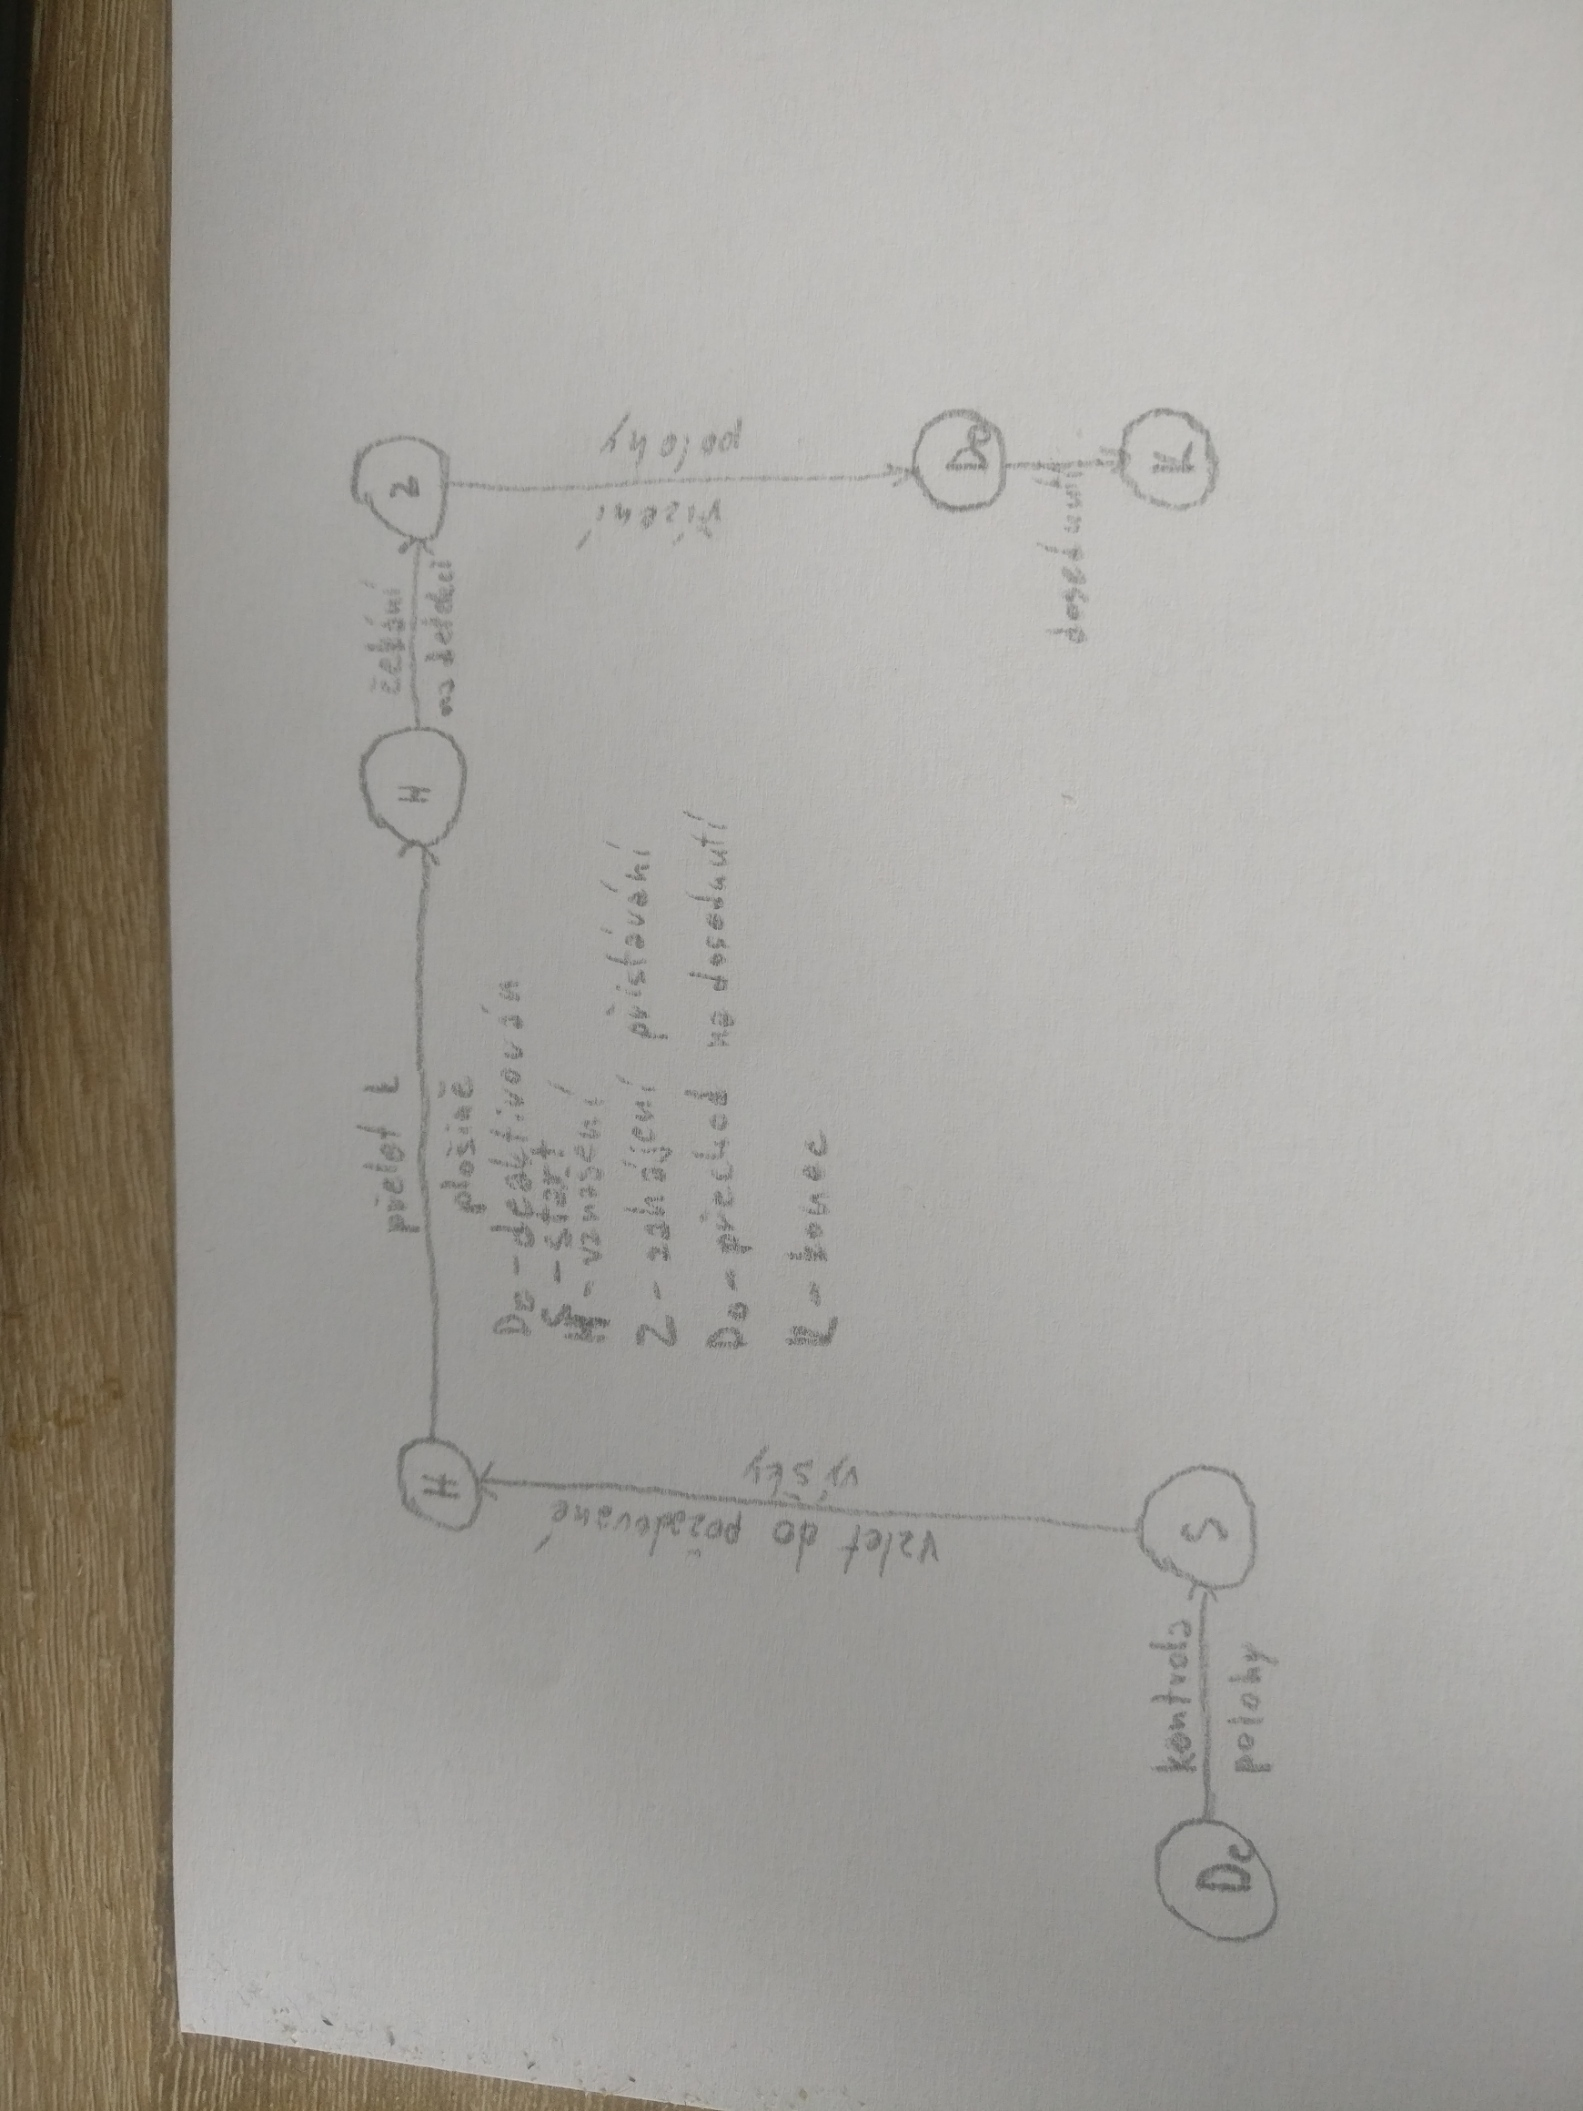
\includegraphics[height=\textwidth,angle=-90,origin=c]{img/algs/genAlg.jpg}
        \caption[Činnosti obecného přistávacího algoritmu]{Činnosti obecného přistávacího algoritmu a jejich posloupnost.} %Pouze ilustrační obrázek, bude překreslen
        \label{fig:algObecny}
    \end{figure}
    
    Na začátku simulace je dron umístěn na zemi a není aktivní. Aby bylo možné simulovat přistání, je s~ním nejprve nutné vzletět, čehož se docílí tak, že se aktivuje a řídicí jednotce se zadá příkaz pro vznesení a přelet do dané výšky. Následně je možné začít přistávání za následujících podmínek:
    \begin{enumerate}
        \item Letoun se vznáší ve vzduchu a je skoro\footnote[1]{Až na drobné nuance způsobené chybami měření palubních senzorů a náhodnými vlivy prostředí.} v~klidu.
        \item Je znám odhad polohy letounu pomocí \acrshort{gps} a \acrshort{imu} je správně kalibrovaná.
        \item Letoun má dostatek energie pro přelet nad plošinu a následné přistání za daných přírodních podmínek.
        \item Okamžitá rychlost $v_o$ a směr větru $\phi_o$ jsou náhodné s~normálním rozdělením $$\begin{bmatrix}
            v_o\\
            \phi_o
        \end{bmatrix} \sim \mathcal{N}\left(\begin{bmatrix}
            v\\
            \phi
        \end{bmatrix}; \begin{bmatrix}
            \sigma_v^2 & 0\\
            0          & \sigma_\phi^2
        \end{bmatrix}\right)$$ filtrované dolní propustí 1. řádu s~časovou konstantou $\tau_v = 1{,}59$ pro rychlost a $\tau_\phi = 4{,}77$ pro směr.
        Parametry normálního rozdělení $v, \phi, \sigma_v$ a $\sigma_\phi$ jsou voleny uživatelem systému pro každé přistání.
        \item Přistávací plošina je částečně zastíněná, podíl zastíněné části je $p_s$ a úhel mezi hranou stínu a severo-jižním směrem je $\theta$.
        \item Je známa přibližná geografická poloha plošiny.
    \end{enumerate}
    Z~těchto podmínek platí 2., 4., 5. a 6. po celou dobu přistávání. Pro přistání je nejprve nutné přeletět do blízkosti přistávací plošiny tak, aby mohla být zachycena kamerou umístěnou na palubě \acrshort{uav}. Řídicí jednotce se tedy zadá příkaz pro vodorovný přelet na známé přibližné umístění plošiny. Je-li po přeletu detekovatelný fiduciární marker plošiny, může se k~ní \acrshort{uav} začít přibližovat. Způsob přibližování je závislý na konkrétní metodě a právě jím se jednotlivé metody liší. Pokud se naopak nepodaří značku detekovat, přistání selhává. Může to být způsobeno příliš velkou nepřesností v~poloze plošiny, příliš velkou svislou vzdáleností od plošiny, nebo příliš velkým větrem, který letoun vychyluje od vodorovné polohy natolik, že tag je mimo zorné pole kamery.

    I~přes rozdíly, které jsou popsány dále, se využívá stejného způsobu ovládání dronu. Konkrétně se jedná PID regulátor rychlosti v~jednotlivých osách podle vzdálenosti od požadované trajektorie a rotace $\psi$ okolo svislé osy (osa $z$) podle odchylky od základního směru (SJ směr, osa $y$). Jeho výstup je prostřednictvím režimu řízení Offboard zaveden do vnitřní kaskády regulátorů řídicí jednotky \acrshort{uav}.
    
    V~následujících podkapitolách (\labelcref{sec:offboardpid,sec:kalmanoffboardpid,sec:offboardpidangle,sec:kalmanoffboardpidangle}) jsou popsány způsoby přiblížení použité v~implementovaných metodách.

    \section{Přistávání po svislé přímce} \label{sec:offboardpid}
        Přistávání po svislé přímce je nejjednodušší z~implementovaných metod přistávání. Spočívá v~tom, že se letoun řídí tak, aby jeho vodorovná vzdálenost od středu plošiny byla během přistávání nulová. Dle velikosti odchylky se řídí rychlost klesání, dokud dron nedosedne na plošinu. Poté je přistávání ukončeno. Požadovaná rychlost klesání se stanoví podle \refskl{eq:vz}{vzorce}, kde $d$ je vodorovná vzdálenost \acrshort{uav} od středu plošiny (případně požadované trajektorie v~dané výšce u~některých jiných metod) a $h$ je výška nad povrchem, ve které se letoun nachází v~daném okamžiku.
        \begin{equation} \label{eq:vz}
            v_z = \frac{1}{2\cdot\left(1+\frac{12\cdot d^2}{h}\right)}
        \end{equation}

        Vzájemná poloha letadla a středu značky je odhadována detektorem zvolených fiduciárních markerů, tedy AprilTagů, na základě obrazových dat z~kamery. Způsob odhadování polohy je podrobněji popsán v~\refskl{chap:detection}{kapitole}. Aby bylo možné relativní vzdálenost určit správně a ve správném měřítku, musí být známá kalibrace kamery a rozměr značky.

        \refskl{eq:vz}{Vztah} byl tímto způsobem stanoven, aby funkce rychlosti byla hladká a v~případě odchylky ji bylo možné korigovat před tím, než fiduciární značka opustí zorné pole kamery a nebude tak možné dále odhadovat polohu plošiny. Pokud by k~tomu i tak došlo (např. vlivem silného poryvu větru), dron bude po omezenou dobu (max. 50 snímků bez tagu) stoupat konstantní rychlostí danou v~konfiguračním souboru (výchozí hodnota je $v_z=0{,}3~\mathrm{m/s}^2$) a čekat na snímek z~kamery, který by obsahoval tag. Nedojde-li k~tomu včas, pokus o~přistání se opakuje od přeletu nad plošinu. % TODO: Dodat číslo kroku v diagramu
        
    \section{Přistávání po svislé přímce s~využitím Kálmánova filtru} \label{sec:kalmanoffboardpid}
        Tento algoritmus je přímo odvozený od předchozího, stejně jako u~něj je požadována nulová vodorovná vzdálenost dronu a plošiny během přistávání a výpočet svislé rychlosti se také neliší. Rozdíl spočívá v~tom, že je sestaven jednoduchý dynamický model letounu, který se následně využívá pro predikci stavu v~Kálmánově filtru \cite{Kalman1960}, \cite{Kalman1961} a měření polohy získaná z~detektoru, která jsou zatížená šumem, se pak filtrují, čímž je dosaženo vyšší přesnosti odhadu polohy. Filtrované odhady se dále používají stejným způsobem jako v~předchozí metodě a je podle nich řízena vodorovná rychlost \acrshort{uav}.

        Pro tyto účely byl letoun modelován lineárním stochastickým systémem diskrétním v~čase jako hmotný bod se směrem rotace, jehož stav je dán polohou v~3D prostoru a rychlostí v~příslušných souřadnicích, uvažovala se také rotace $\psi$ kolem osy $z$ úhlová rychlost $\dot \psi$ v~téže ose. Vstupem systému je požadované zrychlení (nebo úhlové zrychlení) v~jednotlivých proměnných, které je dané řízením dronu. Kromě vstupu na systém dále působí šum s~normálním rozdělením $\mathbf{w} \sim \mathcal{N}(\mathbf{0},\mathbf{Q})$ s~kovarianční maticí $\mathbf{Q}$, která byla určena řádově podobně jako v~\cite{Kojima2015} a dále podle obvyklých kovariancí chyb \acrshort{imu}. %TODO: Dodat zdroj obvvyklých kovariancí
        Vývoj stavu potom určuje \cref{eq:kalmanx}.

        Měření z~uvedeného modelu jsou přímo 3 polohové souřadnice ($x, y, z$) a rotace $\psi$. I~měření je navíc zatíženo náhodnou chybou modelovanou náhodnou veličinou s~normálním rozdělením $\mathbf{v} \sim \mathcal{N}(\mathbf{0},\mathbf{R})$. Jeho kovarianční matice $\mathbf{R}$ byla odhadnuta jako výběrová kovarianční matice měření odchylek relativní polohy měřené detektorem od skutečné relativní polohy v~simulátoru. Měření $\mathbf z$ potom popisuje \cref{eq:kalmanz}.

        Pro fungování Kálmánova filtru je důležitý i vývoj kovarianční matice stavu $\mathbf{P}$ (protože stav je náhodná veličina), kterou je nutné inicializovat pro čas $k=0$. Tato kovarianční matice byla také odhadnuta jako výběrová pro odchylky požadované polohy pro přelet od skutečné polohy po přeletu. Tento způsob odhadu kovarianční matice odpovídá skutečnému průběhu simulace přistávání, jak byla popsána v~\refskl{sec:generalalg}{podkapitole}. Použitý model je tedy dán následujícími rovnicemi:
        \begin{align}
            \mathbf{x}_{k+1} &= \mathbf{Fx}_k + \mathbf{Bu}_k + \mathbf{w}_k,\quad\mathrm{kde} \label{eq:kalmanx} \\
            \mathbf{F} &= \begin{bmatrix}
                1 & \Delta t & 0 &        0 & 0 & 0        & 0 & 0 \\
                0 & 1        & 0 &        0 & 0 & 0        & 0 & 0 \\
                0 & 0        & 1 & \Delta t & 0 & 0        & 0 & 0 \\
                0 & 0        & 0 & 1        & 0 & 0        & 0 & 0 \\
                0 & 0        & 0 & 0        & 1 & \Delta t & 0 & 0 \\
                0 & 0        & 0 & 0        & 0 & 1        & 0 & 0 \\
                0 & 0        & 0 & 0        & 0 & 0        & 1 & \Delta t\\
                0 & 0        & 0 & 0        & 0 & 0        & 0 & 1
            \end{bmatrix}, \quad \mathbf{x}_k = \begin{bmatrix}
                x_k \\ \dot x_k \\ y_k \\ \dot y_k \\ z_k \\ \dot z_k \\ \psi_k \\ \dot\psi_k
            \end{bmatrix}, \quad \nonumber\\
            \mathbf{B} &= \begin{bmatrix}
                \frac{1}{2}\Delta t^2 & 0 & 0 & 0 \\
                \Delta t & 0 & 0 & 0 \\
                0 & \frac{1}{2}\Delta t^2 & 0 & 0 \\
                0 & \Delta t & 0 & 0 \\
                0 & 0 & \frac{1}{2}\Delta t^2 & 0 \\
                0 & 0 & \Delta t & 0 \\
                0 & 0 & 0 & \frac{1}{2}\Delta t^2 \\
                0 & 0 & 0 & \Delta t \\
            \end{bmatrix}, \quad \mathbf{u}_k = \begin{bmatrix}
                \ddot x \\
                \ddot y \\
                \ddot z~\\
                \ddot \psi \\
            \end{bmatrix}, \quad \mathbf{w}_k \sim \mathcal{N}(\mathbf{0},\mathbf{Q}),\quad\mathrm{kde}\nonumber\end{align}\begin{align}
            \mathbf{Q} &= \begin{bmatrix}
                0 & 0       & 0 & 0       & 0 & 0       & 0 & 0\\
                0 & 0{,}002 & 0 & 0       & 0 & 0       & 0 & 0\\
                0 & 0       & 0 & 0       & 0 & 0       & 0 & 0\\
                0 & 0       & 0 & 0{,}002 & 0 & 0       & 0 & 0\\
                0 & 0       & 0 & 0       & 0 & 0       & 0 & 0\\
                0 & 0       & 0 & 0       & 0 & 0{,}004 & 0 & 0\\
                0 & 0       & 0 & 0       & 0 & 0       & 0 & 0\\
                0 & 0       & 0 & 0       & 0 & 0       & 0 & 0{,}02
            \end{bmatrix} \nonumber \\ \nonumber \\
            \mathbf z_k &= \mathbf{Hx}_k + \mathbf{v}_k, \quad \mathrm{kde} \quad \mathbf{v}_k \sim \mathcal{N}(\mathbf{0},\mathbf{R}), \label{eq:kalmanz}\\
            \mathbf H &= \begin{bmatrix}
                1 & 0 & 0 & 0 & 0 & 0 & 0 & 0\\
                0 & 0 & 1 & 0 & 0 & 0 & 0 & 0\\
                0 & 0 & 0 & 0 & 1 & 0 & 0 & 0\\
                0 & 0 & 0 & 0 & 0 & 0 & 1 & 0\\
            \end{bmatrix} \nonumber
        \end{align}
        Mezi aktualizacemi senzorů, jejichž měření jsou do řídicího programu zasílána prostřednictvím protokolu MAVLink, jsou hodnoty veličin považovány za konstantní. Frekvence aktualizací je $\frac{1}{\Delta t} = 30~\mathrm{Hz}$. Tato frekvence je shodná se snímkovou frekvencí použité kamery a je od ní odvozena i délka kroku Kálmánova filtru, která tedy činí $\Delta t=\frac{1}{30}~\mathrm{s}$.
    \section{Přistávání po skloněné přímce} \label{sec:offboardpidangle}
        Tento způsob přistávání také vychází z~prvního zmíněného (\cref{sec:offboardpid}), ale narozdíl od předchozího s~Kálmánovým filtrem (\cref{sec:kalmanoffboardpid}) neupravuje měření relativní polohy, ale požadovanou polohu v~průběhu přistávání.
        
        V~předchozích případech je požadovaná relativní horizontální poloha nulová a požadovaná trajektorie je tedy svislá přímka. V~tomto případě je proměnná a je závislá na výšce, ve které se letoun v~daný okamžik nachází, a na odhadu středních hodnot rotací okolo os $y$ a $x$ během vznášení v~klidu, které jsou dány tím, jak dron překonává síly působené větrným prouděním. Požadovanou trajektorií je přímka s~takovým sklonem, aby pro dané rotace (a tím i pro danou rychlost a daný směr větru) kamera \acrshort{uav} mířila na střed přistávací plošiny. Rychlost se v~závislosti na odchylce od požadované trajektorie vypočte stejným způsobem jako v~předchozích případech, tedy dle \refskl{eq:vz}{vztahu}.

        \begin{figure}
            \centering
            \begin{tikzpicture}
                \begin{axis}[
                  view={42}{23},
                  axis lines=center,
                  width=15cm,height=12cm,
                  xtick={-1,1,2,3},ytick={-1,1,2,3},ztick={-1,5,10},
                  minor tick={-12,-11,...,12},
                  xmin=-1.5,xmax=3.5,ymin=-1.5,ymax=3.5,zmin=-2,zmax=7,
                  xlabel={$x$},ylabel={$y$},zlabel={$z$},
                ]
                \addplot3[mesh, gray!40, domain=-1:3, samples=5, domain y=-1:3, samples y=5, forget plot] {0};
                
                % plot dots for the two points
                
                
                % plosina
                \addplot3 [no marks] coordinates {(-0.35,-0.35,0) (0.35,-0.35,0) (0.35,0.35,0) (-0.35,0.35,0) (-0.35,-0.35,0)};
                \path (axis cs:0,0,0) coordinate (O) (axis cs:1,0,0) coordinate (X) (axis cs:0,1,0) coordinate (Y) (axis cs:0,0,1) coordinate (Z) (axis cs:0,0,0) coordinate (P) [x={($(X)-(O)$)},y={($(Y)-(O)$)},z={($(Z)-(O)$)}, canvas is xy plane at z=0,transform shape,rotate=180] (P) node{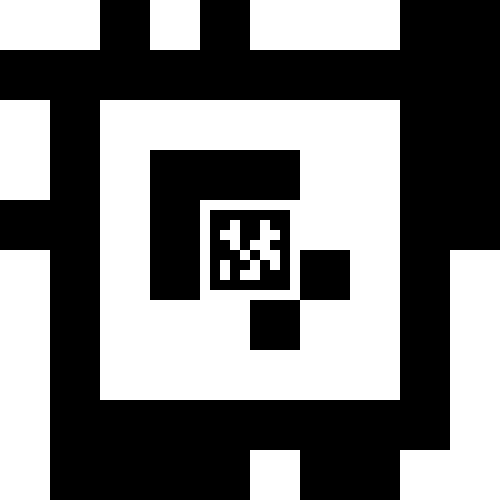
\includegraphics[width=0.7cm,height=0.7cm]{img/tag_48_12__36_11_164__137.png}};

                % trajectory
                \addplot3 [no marks, densely dashed, red] coordinates {(0,0,0) (1.4,0.7,7)};

                \addplot3 [no marks, densely dashed, gray] coordinates {(0,0,0) (3.5,1.75,0)};
                \addplot3 [no marks, densely dashed, gray] coordinates {(1,0.5,5) (1,0.5,0)};

                % drone
                \addplot3 [] coordinates {(1.174574312188794, 0.587287156094397, 4.956356421952801) (0.8254256878112061, 0.41271284390560303, 5.043643578047199)};
                \addplot3 [] coordinates {(1.0894427190999916, 0.32111456180001685, 5.0) (0.9105572809000084, 0.6788854381999831, 5.0)};
                \addplot3 [only marks,mark=halfsquare*,mark size = 1.5pt] coordinates {(1,0.5,5)};

                \addplot3 [gray, densely dotted, line width=0.25mm] coordinates {(1.174574312188794, 0.587287156094397, 0) (0.8254256878112061, 0.41271284390560303, 0)};
                \addplot3 [gray, densely dotted, line width=0.25mm] coordinates {(1.0894427190999916, 0.32111456180001685, 0) (0.9105572809000084, 0.6788854381999831, 0)};
                
                % label points
                \node [above right] at (axis cs:1,0.5,5) {\acrshort{uav}};
                \node [inner sep=2pt,outer sep=0pt] (O) at (axis cs:0,0,0) {};
                \node [align=center] (plosinatext) at ([xshift=1.5cm,yshift=-1.8cm]O) {Plošina};
                \draw [shorten <=.1cm,stealth-,gray] (O) to [out=-30,in=160] (plosinatext.west);

                \node [inner sep=0pt,outer sep=0pt] (A) at (axis cs:3,1.5,5) {};
                \node [inner sep=0pt,outer sep=0pt] (B) at (axis cs:2,1,5) {};

                \draw [-stealth] (A) -- (B) node [midway, above, sloped] {směr větru};
                \addplot3 [lightgray, densely dotted] coordinates {(3,1.5,5) (3,1.5,0)};
                \addplot3 [lightgray, densely dotted] coordinates {(2,1,5) (2,1,0)};
                \addplot3 [lightgray, densely dotted] coordinates {(2,1,5) (0,0,5)};

                \end{axis}
                \end{tikzpicture}
            \caption[Přistávání po skloněné přímce]{Přistávání po skloněné přímce (červeně). Letadlo je nakloněné proti větru, čímž ho překonává a zároveň kamerou míří na střed plošiny, která je tak v~zorném poli i za přítomnosti poruch.}
            \label{fig:offboardpidangle}
        \end{figure}
        

        Tato metoda má za cíl zlepšit podmínky pro detekci značky na plošině při působení silného větru. V~případě nutné korekce nějaké poruchy (způsobené například poryvem větru) zbývá okolo tagu více místa v~obrazu, kam se může posunout, aniž by opustil zorné pole a tím znemožnil odhadovat svoji polohu vůči letounu.
    \section{Přistávání po skloněné přímce s~využitím Kálmánova filtru} \label{sec:kalmanoffboardpidangle}
        Poslední implementovaný přístup využívá obou změn navržených v~předchozích dvou upravených metodách (\cref{sec:kalmanoffboardpid,sec:offboardpidangle}). Pro odhad vzájemné polohy dronu a značky na přistávací plošině je aplikován Kálmánův filtr s~měřeními z~detektoru tagů a lineárním stochastickým systémem jako modelem pohybu a rotace dronu v~prostoru. Stejně jako ve všech implementovaných metodách pro přistávání je tento odhad využit PID regulátorem, který řídí požadovanou rychlost \acrshort{uav} ve dvou vodorovných osách tak, aby byla následována požadovaná trajektorie, a jeho výstup je zapojený do interní kaskády regulátorů řídicí jednotky letounu. V~tomto případě je základní svislá trajektorie nahrazena skloněnou trajektorií proti směru větru, aby i při jeho překonávání letounem zůstala značka na plošině uprostřed zorného pole kamery, jak již bylo popsáno v~předchozí podkapitole. Všechny tyto popsané metody byly podrobeny experimentům za různých podmínek a byla vyhodnocena jejich úspěšnost, přesnost a další vlastnosti. Popis těchto experimentů je v~\refskl{chap:eval}{kapitole}.